\documentclass[12pt]{article}
\usepackage[utf8]{inputenc}
\usepackage[letterpaper, margin=1in]{geometry}
\usepackage{graphicx}
\usepackage{mathptmx}
\usepackage{float}
\usepackage[cmex10]{amsmath}
\usepackage{amsthm,amssymb}
\usepackage{url}
\urlstyle{same} 
\def\UrlBreaks{\do\/\do-}
\usepackage{breakurl}
\usepackage{fancybox}
\usepackage{breqn}
\usepackage{array}
\usepackage{caption}
\usepackage{subcaption}
\usepackage{comment}
\usepackage[english]{babel}
\usepackage[acronym,nomain]{glossaries} % list of acronyms
\usepackage{xurl}
\usepackage{cite} % math and engineering style citations
\usepackage{multicol}
\usepackage{multirow}
\usepackage{mathptmx}
\usepackage{float}
\usepackage{lipsum}
\usepackage{framed}
\usepackage{empheq}
\usepackage[T1]{fontenc}
\usepackage[pdfpagelabels,pdfusetitle,colorlinks=false,pdfborder={0 0 0}]{hyperref}

\renewcommand{\arraystretch}{1.2}

\sloppy

\newcolumntype{C}[1]{>{\centering\let\newline\\\arraybackslash\hspace{0pt}}m{#1-2\tabcolsep}}

\title{Charging Network Optimization with Nonlinear Station Size Effects}
\author{Aaron Rabinowitz}
\date{}

\newacronym{good}{GOOD}{Grid Optimized Operation Dispatch}
\newacronym{od}{OD}{Economic Dispatch}
\newacronym{ce}{CE}{Capacity Exapnsion}
\newacronym{soc}{SOC}{State of Charge}
\newacronym{mud}{MUD}{Multi-Unit Dwelling}
\newacronym{bev}{BEV}{Battery Electric Vehicle}
\newacronym{ess}{ESS}{Energy Storage System}
\newacronym{icev}{ICEV}{Internal Combustion Engine Vehicle}
\newacronym{frp}{FRP}{Flow Refueling Problem}
\newacronym{esn}{ESN}{Energy Supply Network}
\newacronym{afdc}{AFDC}{Alternative Fuels Data Center}
\makeglossaries

\begin{document}

\maketitle

\section{Queuing at Stations}

\begin{figure}[H]
	\centering
	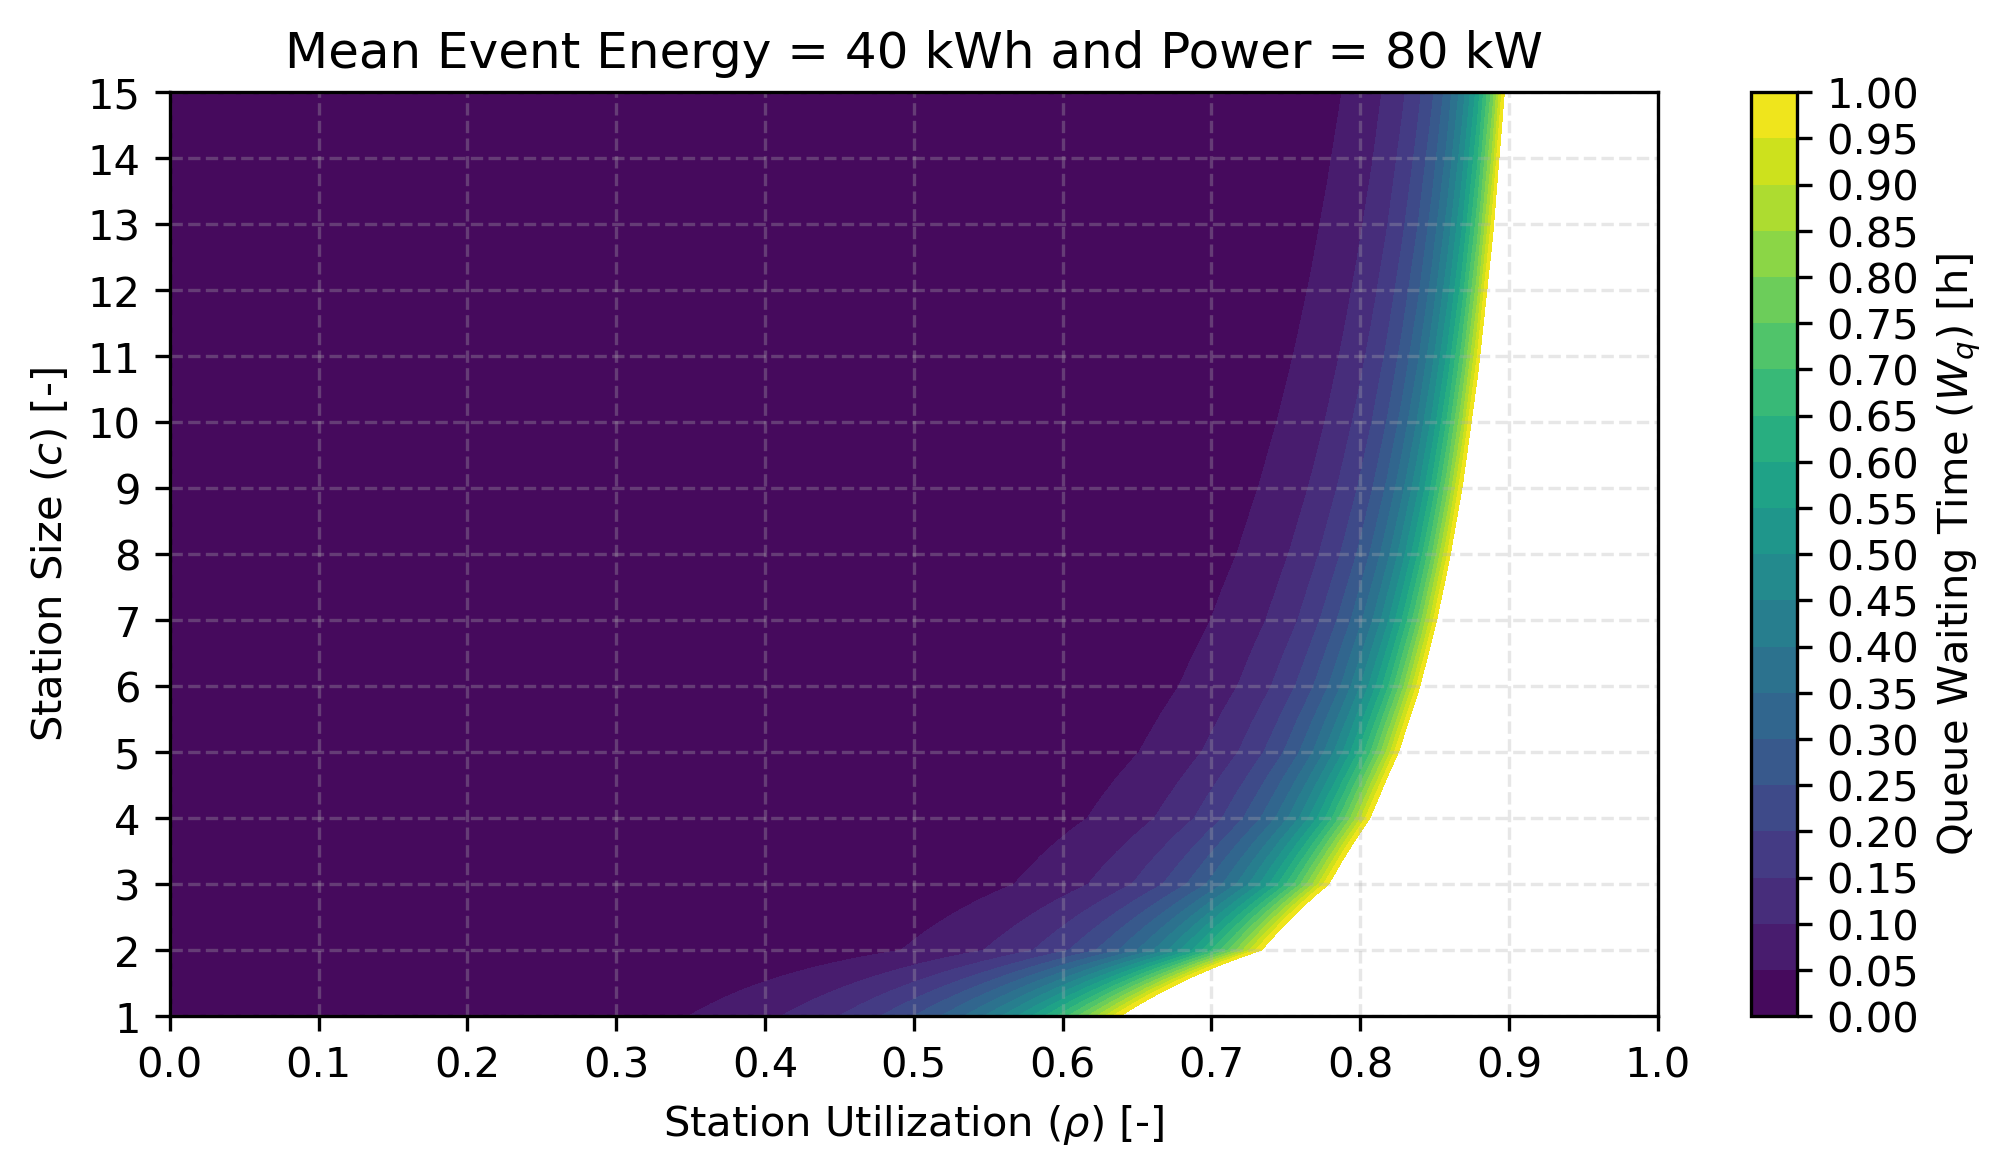
\includegraphics[width = .7\linewidth]{figs/queue.png}
	\caption{Queuing time with M/M/c queue model}
	\label{fig:queue}
\end{figure}


\section{Travel Time Minimization Formulation}

The purpose of this formulation is to minimize total travel time in the system. Travel time minimization is accomplished by vehicle routing and charging station provision. For a given O/D pair there will, usually, be multiple viable charging paths of different lengths. As demand increases, chargers become increasingly congested leading to queuing time at stations. Queuing delays on shorter paths will push traffic to longer paths. Eventually, queuing will be sufficient to make the charging network no longer beneficial. This point is defined as when the marginal vehicle trip would take as much time using the network as it would take using level 1 charging. The goal is to place chargers and route vehicles to minimize total ravel time. As such, each O/D pair has a "failure" flow which vehicles can be assigned to and the penalty assigned for this is equal to the travel time with level 1 charging.

Delay at stations is modeled using the outputs of the M/M/c queue formula as discussed in Section [REF]. Specifically, the outputs are linearized. Stations are initialized with a vector of $m$ binary variables representing possible sizes (e.g. 1 charger, 3 chargers, 5 chargers). The vector of station size binary variables must sum to 1. For each size considered, the M/M/c model returns volumes and delays corresponding to a set of marginal utilization rates $R: |R| = n$. The utilization rates $\rho \in R$ are the bounds of a set of $n - 1$ utilization intervals. Thus, $m$ by $n - 1$ matrices of marginal volumes and marginal delays are created. Additionally, a $m$ by $n$ matrix of unit-interval continuous variables are created and the sum of these variables multiplied by the corresponding marginal volumes must equal the flow passing through the station. the delay at the station is computed by summing the marginal utilization rates multiplied by the marginal delays.

\begin{itemize}
	\item $G = \{V, E\}$: System graph containing nodes $v \in V$ and edges $(i, j) \in E$. Edge costs are defined by the following sets: \begin{itemize}
		\item $Y^T$: The time required to traverse edge $(i, j)$
		\item $Y^E$: The time required to charge at node $i$ to successfully traverse edge $(i, j)$
	\end{itemize}
	\item $O \subseteq V$: Set of origin nodes
	\item $D \subseteq V$: Set of destination nodes
	\item $S \subseteq V$: Set of nodes with charging stations (or the possibility of a station). Stations provide energy to vehicle flows at a given rate. Depending on the utilization level of the station, vehicles may experience delay. The relationship between utilization is linearized using the following sets: \begin{itemize}
		\item $C_s$: Set of possible station sizes at station $s \in S$
		\item $K_{s, c}$: Set of capacity intervals at station $s \in S$ for station size $c \in C_s$
		\item $Y^V$: Set of volumes corresponding to each $c \in C_s$ and $k \in K_s$
		\item $Y^D$: Set of delays corresponding to each $c \in C_s$ and $k \in K_s$ 
	\end{itemize}
	\item $\hat{C}$: Maximum number of chargers which can be installed
	\item $Q$: Set of demand tuples of the form $\langle o, d, v, c, \hat{t} \rangle$ where $o$ is the origin, $d$ is the destination, $v$ is the volume, $c$ is the capacity of the \gls{ess} capacity of vehicles, and $\hat{t}$ is the maximum travel time that is acceptable for the given demand. \begin{itemize}
		\item $Y^Q$: Set of time penalties for failing to accommodate flow. Set so that $y^q_q$ is equal to $\hat{t}$ in $q$.
	\end{itemize}
	\item $P$: Set of paths corresponding to each demand $q \in Q$. Paths begin at $o \in O$ and end at $d \in D$. All intermediate nodes $i \in P \setminus \{o, d\}$ must be stations $s \in S$.\begin{itemize}
		\item $P^q$: Paths that correspond to demand $q \in Q$
		\item $P^s$: Paths that include station $s \in S$
	\end{itemize}
	\item $X$: Set of continuous decision variables: \begin{itemize}
		\item $X^Q$: Portion of demand flow not facilitated by the network
		\item $X^P$: Flow volumes along paths
		\item $X^U$: Portion of station capacity intervals utilized
		\item $X^V$: Volume seen at station
		\item $X^D$: Queuing delay seen at station
	\end{itemize}
	\item $U$: Set of integer decision variables: \begin{itemize}
		\item $U^S$: Booleans for station sizes corresponding to $S$ and $C$
	\end{itemize}
\end{itemize}


The objective of the optimization is

\begin{gather}
	\min_{\overline{X},\overline{U}}\quad \underbrace{\sum_{q \in Q} x^q_qy^q_q}_{\text{Penalty Time}} + \underbrace{\sum_{q \in Q}\sum_{P^q \in P}\sum_{p \in P^q}\sum_{(i, j) \in p} x^p_p(y^t_{(i, j)} + y^e_{(i, j)})}_{\text{Edge Traversal Time}} + \underbrace{\sum_{s \in S}\sum_{c \in C_s}
	\sum_{k \in K_{s, c}} u^s_{s, c}x^u_{s, c, k}y^d_{s, c, k}}_{\text{Queuing Time}} \label{eq:tm:obj}
\end{gather}

subject to

\begin{gather}
	Q[v] - x^q_q - \sum_{p \in P^q}x^p_p = 0 \quad \forall q \in Q \label{eq:tm:flow_dem} \\
	\sum_{p \in P^s} x^p_p - \sum_{c \in C_s}
	\sum_{k \in K_{s, c}} u^s_{s, c}x^u_{s, c, k}y^v_{s, c, k} = 0 \quad \forall s \in S \label{eq:tm:flow_cons} \\
	x^u_{s, c, k} - u^s_{s, c} \leq 0 \quad \forall s \in S, \ \forall c \in C_s,\ \forall k\in K_{s, c} \label{eq:tm:sz_int} \\
	\sum_{c \in C_s} u^s_{s, c} - 1 = 0 \quad \forall s \in S \label{eq:tm:chg_unity} \\
	\sum_{s \in S}\sum_{c \in C_s} u^s_{s, c} - \hat{C} \leq 0 \label{eq:tm:chg_tot}
\end{gather}

The objective function \eqref{eq:tm:obj} minimizes total travel time in three terms. The first term is the time penalties accrued for failing to accommodate demand. The theory is that, without dedicated charging infrastructure, vehicles could, theoretically, complete the trip using level 1 charging but this would be very slow if the trip is beyond full-charge range. The second term is the time spent driving along edges and charging to drive along edges. The third term is the time spend queuing for a charger. Constraint \eqref{eq:tm:flow_dem} forces the sum of flows and un-accommodated flows to be equal to total demand. Constraint \eqref{eq:tm:flow_cons} forces the sum of utilization intervals at a station to be equal to the sum of flows which pass through the station. Constraint \eqref{eq:tm:sz_int} forces station utilization to only accrue for the selected station size. Constraint \eqref{eq:tm:chg_unity} forces only one station size to be selected per station and \eqref{eq:tm:chg_tot} limits the total number of chargers in the network.

%\section{Description}
%
%Consider a \gls{mud} with a parking lot containing $N$ assigned spaces with AC chargers serving a set of $V$ vehicles. The chargers at these N spaces each have a maximum charging rate of $R$. The $N$ chargers are all on the same circuit. The circuit has a maximum power of $P$. The chargers are managed by a charge management system which has knowledge of vehicle itineraries and \glspl{soc}. The charge management system can assign rates to the vehicles for time intervals where they are plugged in as long as these rates are not higher than $R$ for any individual vehicle and not higher than $P$ for all $N$ vehicles combined.
%
%\section{Optimization Formulation}
%
%The goal of the optimization is to set charging rates for each vehicle and time-step in order minimize the amount of charging which takes place out-of-home while meeting the energy requirements of itineraries. Each vehicle has an itinerary composed of a set of events at evenly-spaced time-steps $T = \{t_0, t_1, \dots, t_m\}$ with corresponding energy consumption values $E^v = \{e^v_0, e^v_1, \dots, e^v_m\}$ representing driving energy for each vehicle $v \in V$. At each time interval each vehicle has a status of not plugged-in $S^{n, v} = \{e^{n, v}_0, e^{n, v}_1, \dots, e^{n, v}_m\}$, plugged-in at home $S^{h, v} = \{e^{h, v}_0, e^{h, v}_1, \dots, e^{h, v}_m\}$, or plugged-in  out-of-home $S^{o, v} = \{e^{o, v}_0, e^{o, v}_1, \dots, e^{o, v}_m\}$. These statuses are mutually exclusive for each time-step. Each vehicle may charge whenever it is plugged in $X^v = \{x^v_0, x^v_1, \dots, x^v_m\}$ and this is the optimization variable. \gls{soc} $L^v = \{l^v_0, l^v_1, \dots, l^v_m\}$ is determined by $E$ and $X$ and must be maintained between 0 and 1. \\
%
%The objective is to minimize overall out-of-home charging for all vehicles and times.
%
%\begin{equation}
%	\min_{\overline{X}} \sum_{v \in V}\sum_{t \in T} x^v_t s^{o, v}_t
%\end{equation}
%
%subject. to
%
%\begin{gather}
%	l^v_t = l^v_{t - 1} - e^v_t + x^v_t\quad  \forall\ v \in V,\ t \in \{t_1, t_2, \dots, t_m\} \\
%	0 \leq l^v_t \leq 1 \quad  \forall\ v \in V,\ t \in T \\
%	l^v_{0} = l_v{1} = 0.5 \quad  \forall\ v \in V \\
%	0 \leq \sum_{v \in V} x^v_t s^{h, v}_t \leq P\quad \forall\ t\in T \\
%	0 \leq x^v_t s^{h, v}_t \leq R\quad  \forall\ v \in V,\ t\in T \\
%	x^v_t s^{n, v}_t = 0\quad  \forall\ v \in V,\ t\in T \\
%	s^{n, v}_t + s^{h, v}_t + s^{o, v}_t = 1\quad  \forall\ v \in V,\ t\in T \\
%	s^{n, v}_t, s^{h, v}_t, s^{o, v}_t \in \mathbb{Z} \forall\ v \in V,\ t\in T
%\end{gather}
%
%\section{Scenario}
%
%From eVMT data, out of 67 multi-month long \gls{bev} itineraries, 6,484 unique Monday-to-Monday itineraries were samples. These itineraries had driving distances as shown in \ref{fig:1}.
%
%\begin{figure}[H]
%	\centering
%	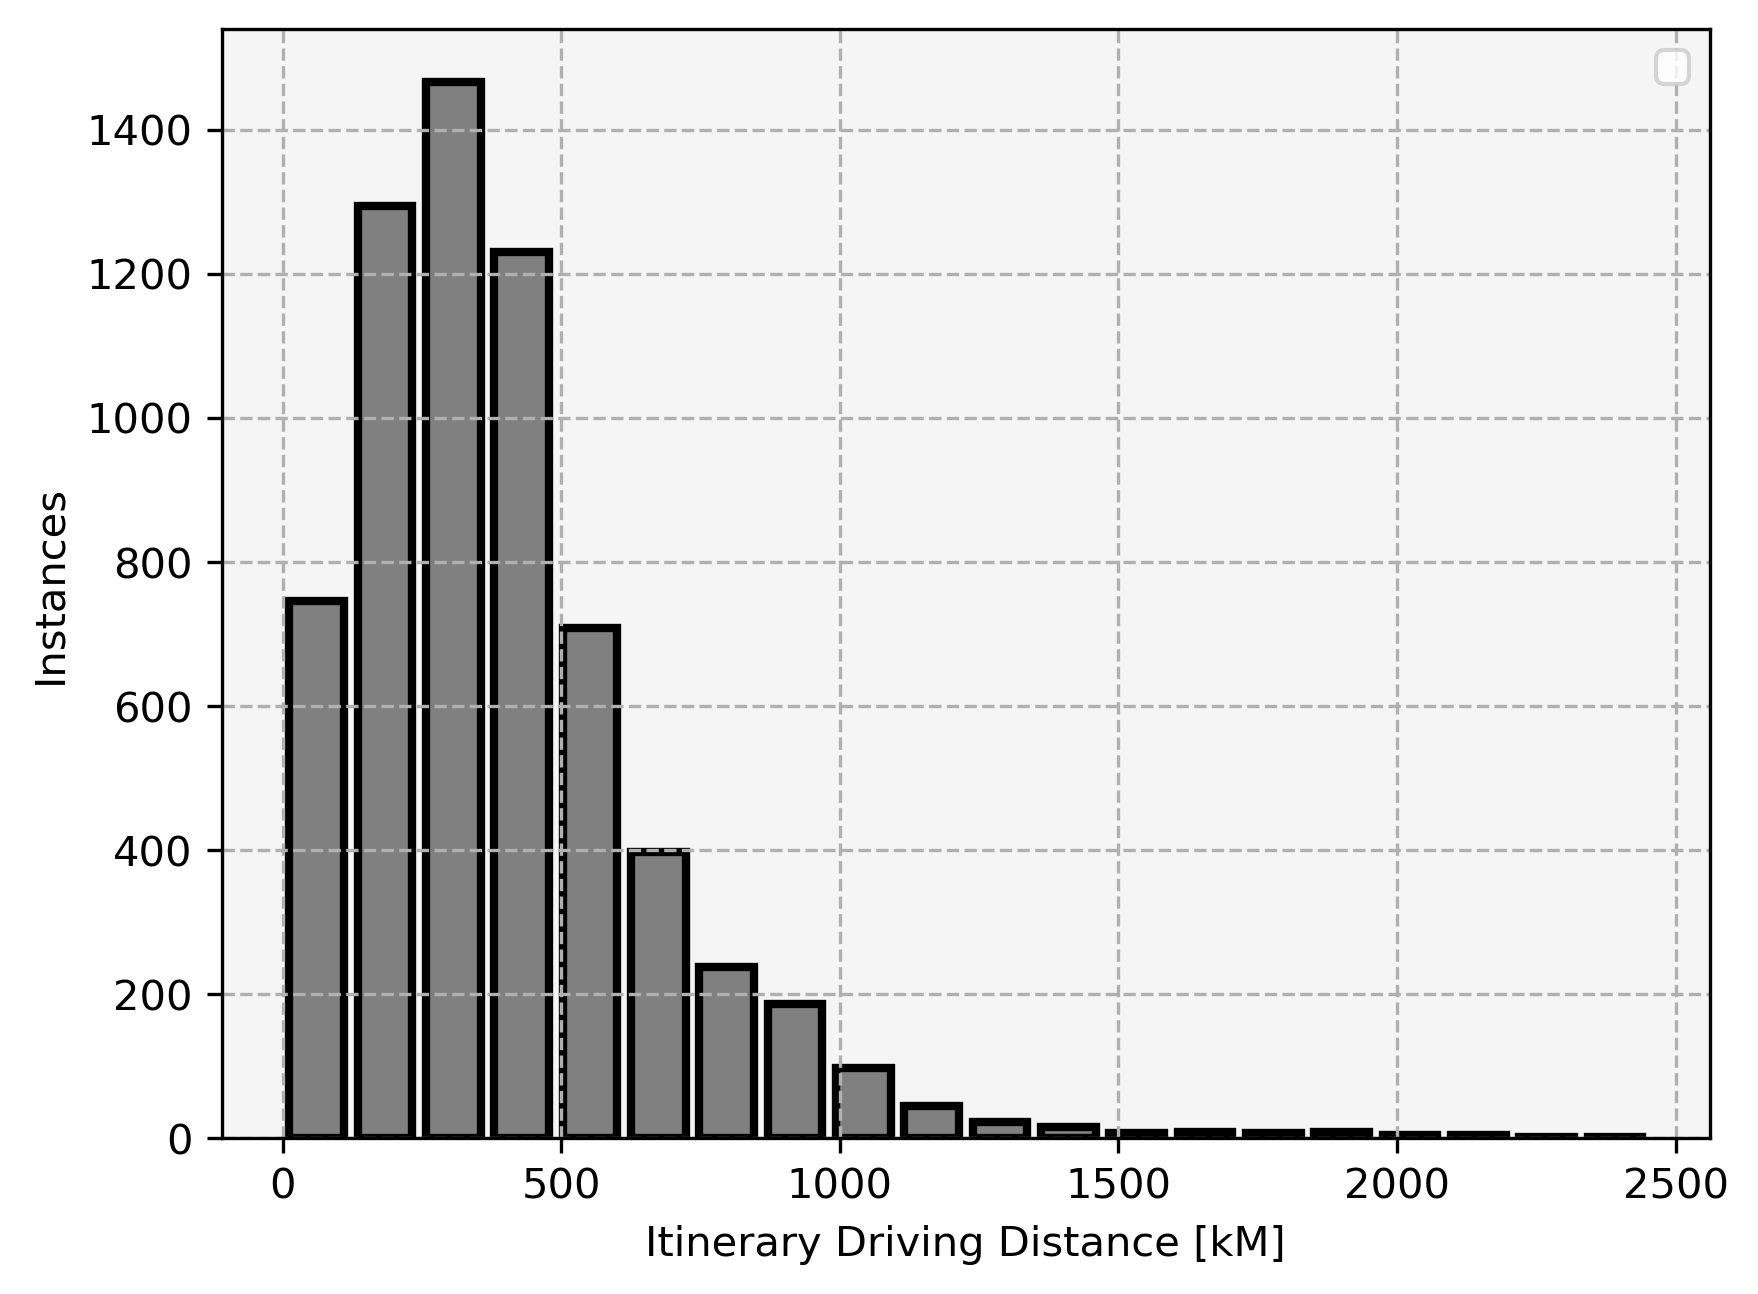
\includegraphics[width = .7\linewidth]{figs/p1.png}
%	\caption{Weekly itinerary total driving distance from dataset}
%	\label{fig:1}
%\end{figure}
%
%These itineraries were used to form 1,000 randomly sampled groups of 8. The vehicles in each group of 8 were assigned battery capacities from standard ranges (triangular distribution (60 - 80 - 100 kWh)). Optimization time intervals were 15 minute periods. Each sampled group of vehicles was considered under two scenarios based on home charging limitations:
%
%\begin{enumerate}
%	\item $R = 3.3$ [kW] and $P = 16$ [kW]
%	\item $R = 8.3$ [kW] and $P = 16$ [kW]
%\end{enumerate}
%
%The constraints above represent a scenario where a 3.3 kW dedicated connection is available to each of the 8 vehicles in the group versus 8 vehicles sharing a total of 16 kW. However, since vehicles are unlikely to be able to accept 16 kW alone, an 8.3 kW vehicle acceptance rate was imposed on each vehicle.
%
%Charging deficit is the amount of charging out-of-home required across all eight vehicles. Results from these scenarios showed that charging deficit was lower in scenario 2 than scenario 1 in 358 out of 1000 cases and the opposite never occurred. The distribution of charging deficit by scenario is shown in \ref{fig:2}.
%
%\begin{figure}[H]
%	\centering
%	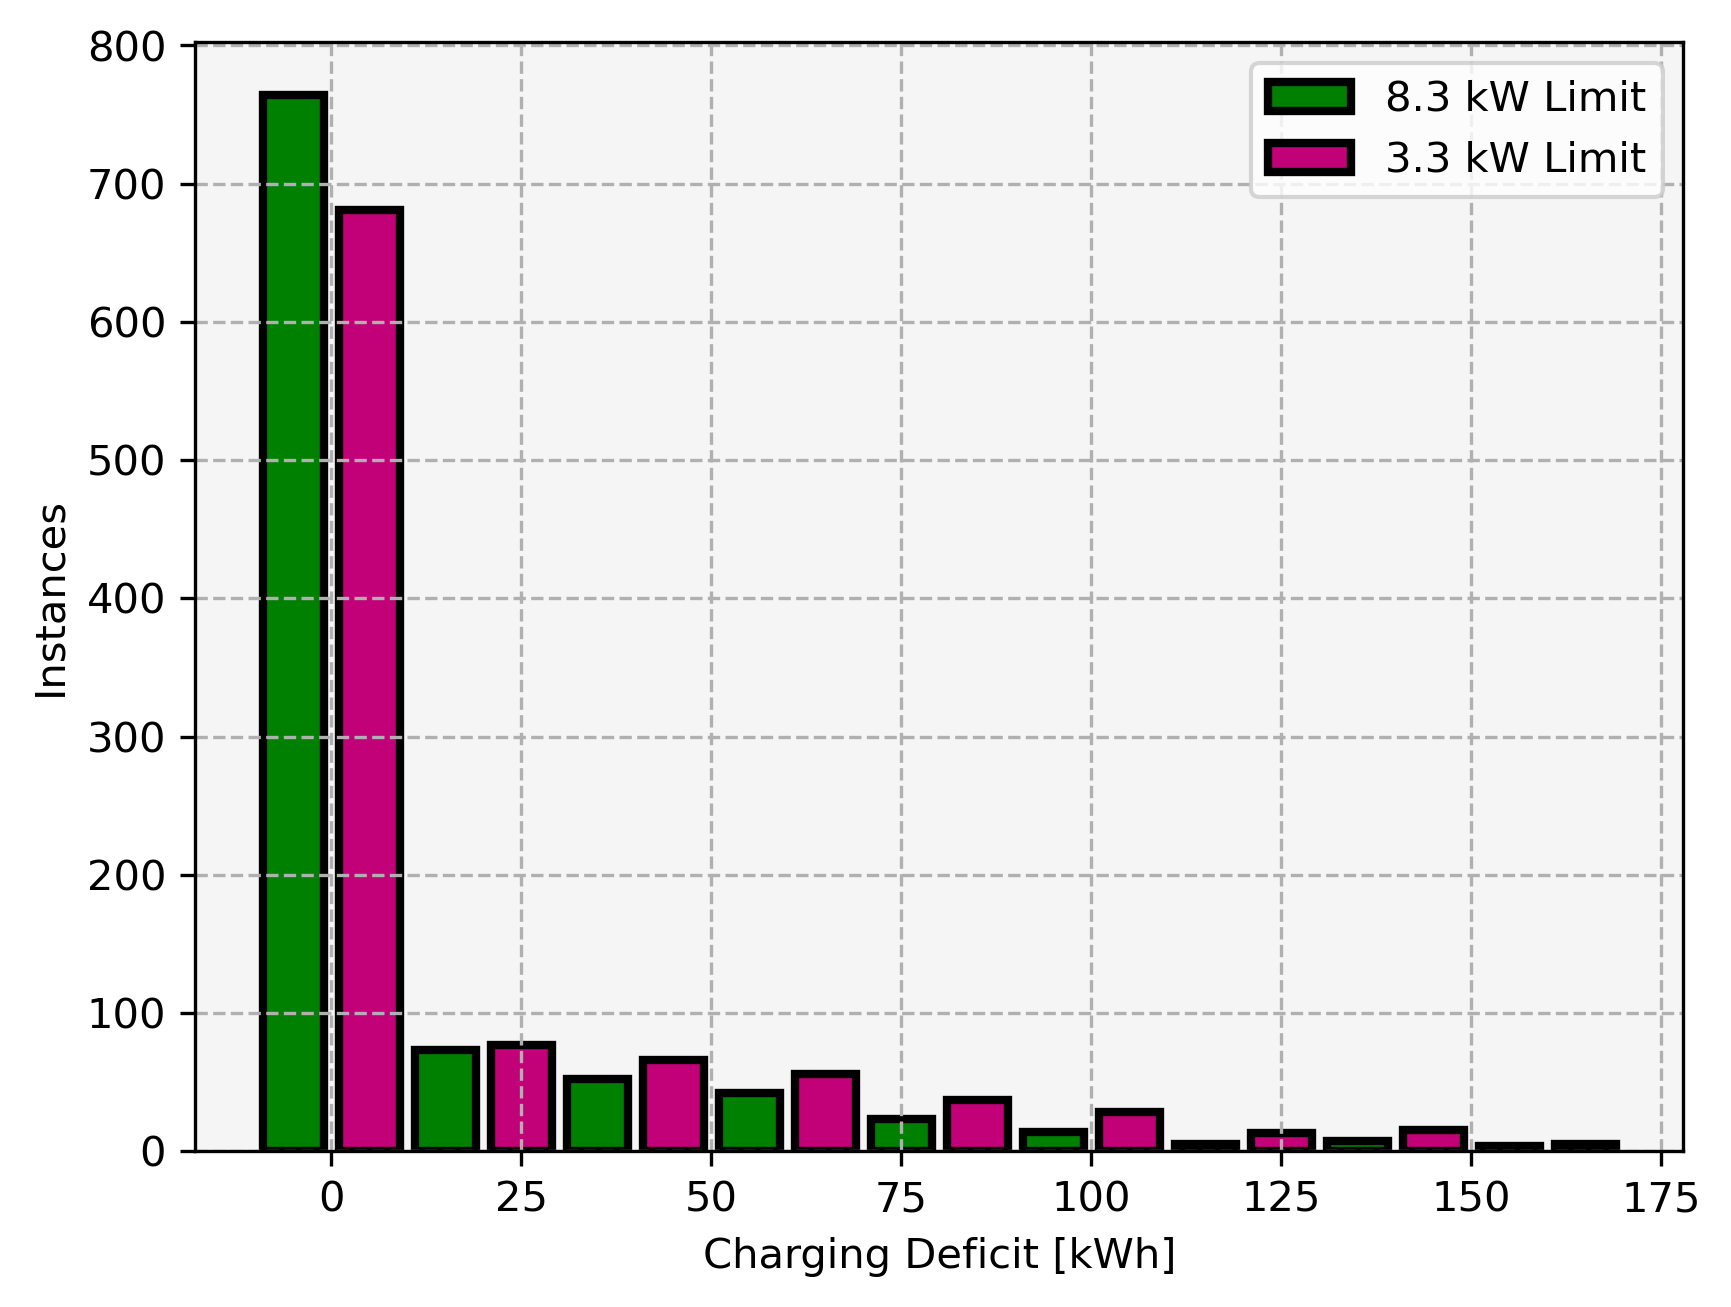
\includegraphics[width = .7\linewidth]{figs/p2.png}
%	\caption{Aggregate charging deficit histogram}
%	\label{fig:2}
%\end{figure}
%
%Charging deficit can also be considered for each driver in the eight individually. The distribution of the number, out of eight, of drivers having a non-zero charging deficit is shown in \ref{fig:3}.
%
%\begin{figure}[H]
%	\centering
%	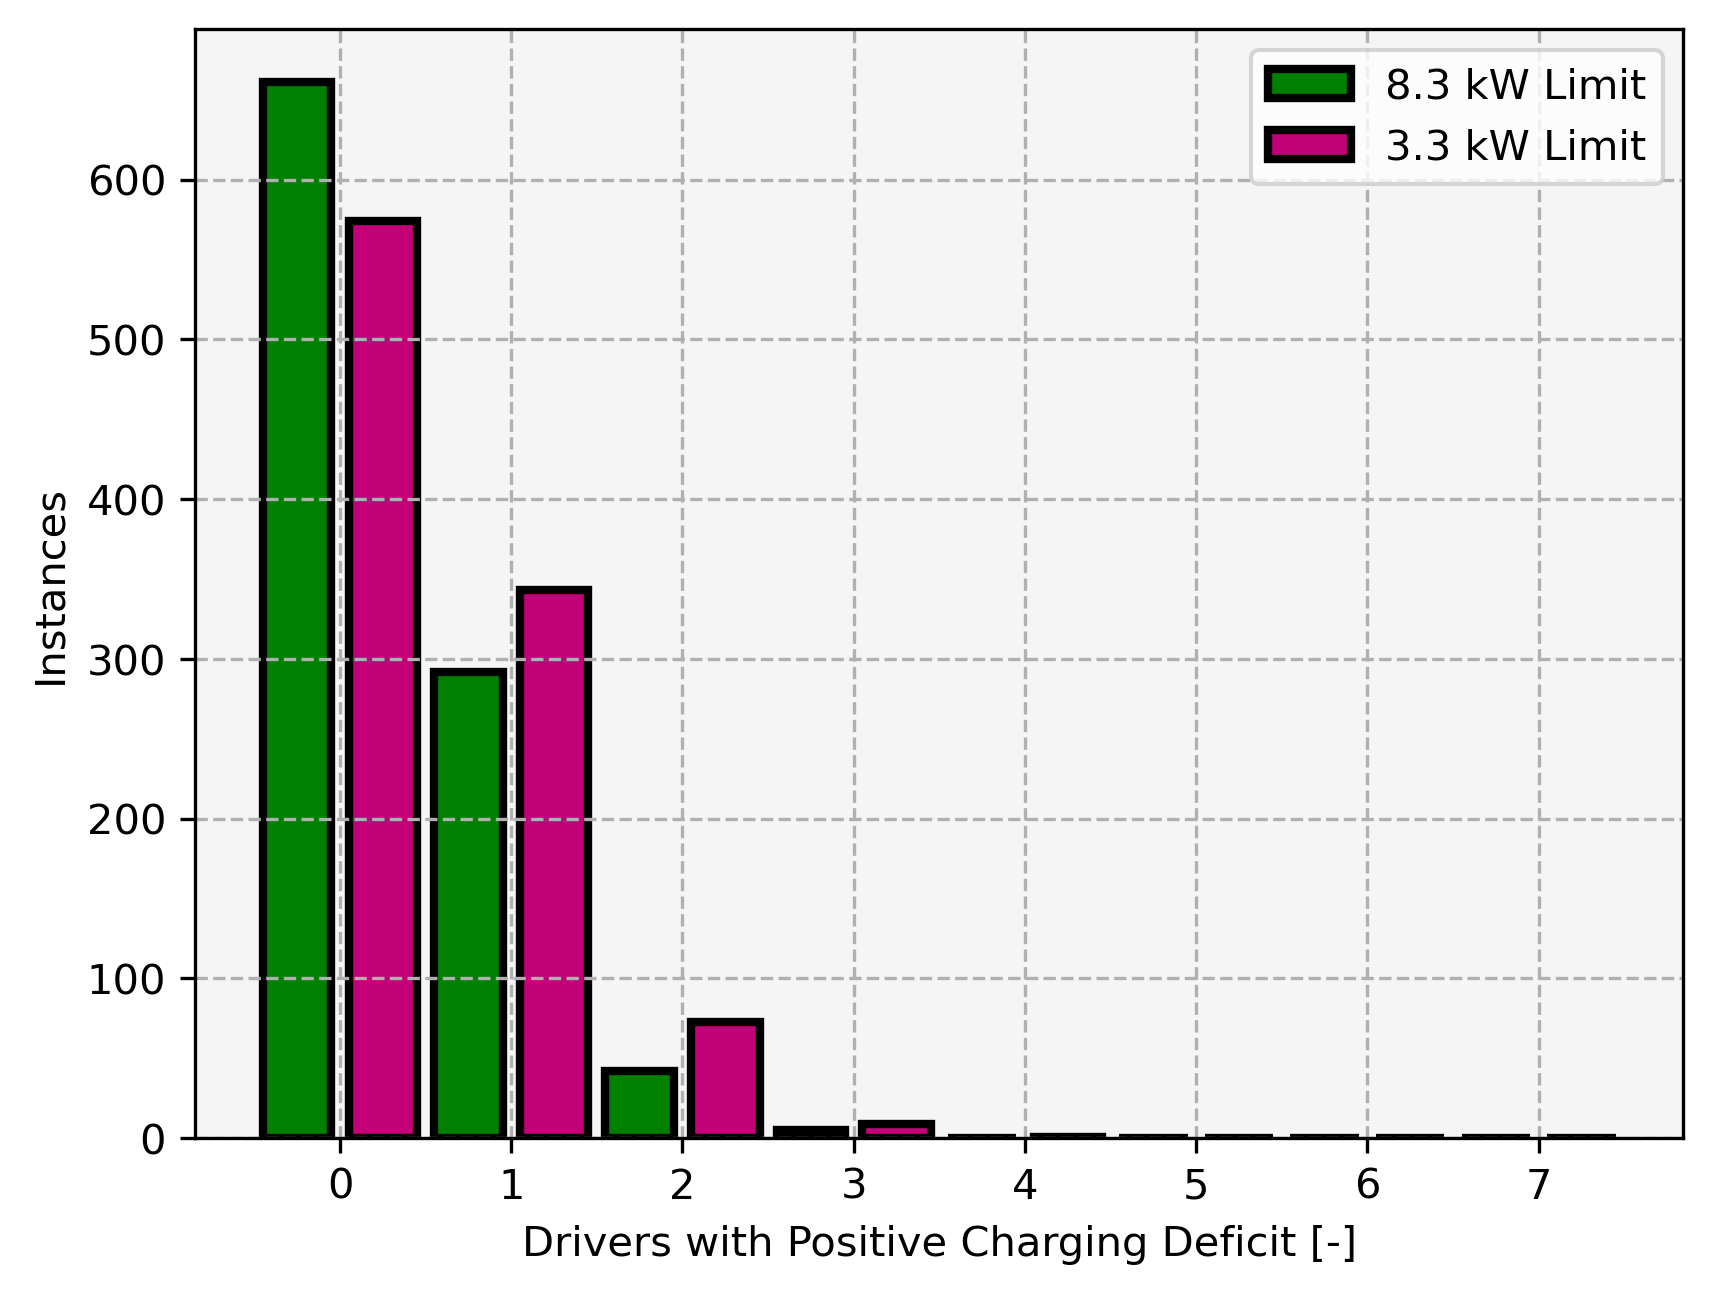
\includegraphics[width = .7\linewidth]{figs/p4.png}
%	\caption{Individual non-zero charging deficit histogram}
%	\label{fig:3}
%\end{figure}
%
%The distributions show a scholastically dominant benefit for scenario 2.


\end{document}